\chapter{自适应的极大二分团枚举数据结构}
\label{ch:adapt_mbe}

针对极大二分团枚举问题中单一数据结构低效的问题,本章整理了相关工作中所涉及的不同的图存储数据结构,详细描述不同数据结构的优劣以及适用场景,并指出单一数据结构所导致的局限性,作为本章的研究动机。具体而言,现有算法通常采用邻接表结构存储二分图,在进行大量集合交集运算时会带来较高的计算开销;同时,过多地访问顶点的全部邻居也存在冗余计算问题。这些因素限制了算法只能应用于包含不超过1亿极大二分团的小数据集。为了解决这些问题,本章提出以下优化方法:首先,针对邻接表上集合运算的高开销问题,本章提出基于位图的动态子图方法。该方法在计算过程中动态生成子位图,通过在子位图中进行集合运算,提升集合运算的效率。然后,针对访问顶点完整邻居导致的冗余计算问题,本章提出局部邻居缓存方法。该方法通过动态保存顶点的部分活跃邻居,避免大量对结果无影响的不活跃邻居的访问,从而减少冗余计算。此类冗余计算包括对含有非极大二分团的节点的计算、重复的集合运算以及无效顶点的访问。最后,本章结合基于位图的动态子图方法和局部邻居缓存方法,形成自适应的极大二分团枚举算法AdaMBE。实验证明,AdaMBE算法相比于现有工作的运行时间缩短1.6-49.7倍,并成功应用于超过190亿极大二分团的TVTropes数据集。

\section{二分图的存储结构}

二分图的存储结构对极大二分团枚举算法中集合运算的效率具有直接影响,在极大二分团枚举过程中扮演着关键角色。图~\ref{fig:ada_graph_format}展示了图~\ref{fig:ada_eg_tree}中二分图$G_2$的三种二分图存储结构,包括邻接表、位图和哈希表。每种数据结构在时间和空间开销上都有其独特的优势和局限性,因此在实际应用中需要权衡各种因素,选择最适合的存储结构解决问题。

\begin{figure} [H]
  \centering
  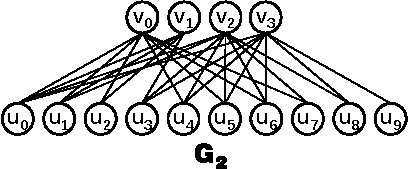
\includegraphics[width=0.5\linewidth]{adambe/eg_graph.pdf}
  \caption{二分图$G_2$}
  \label{fig:ada_eg_tree}
\end{figure}


\begin{figure} [H]
	\centering
  \vspace{0.1in}
	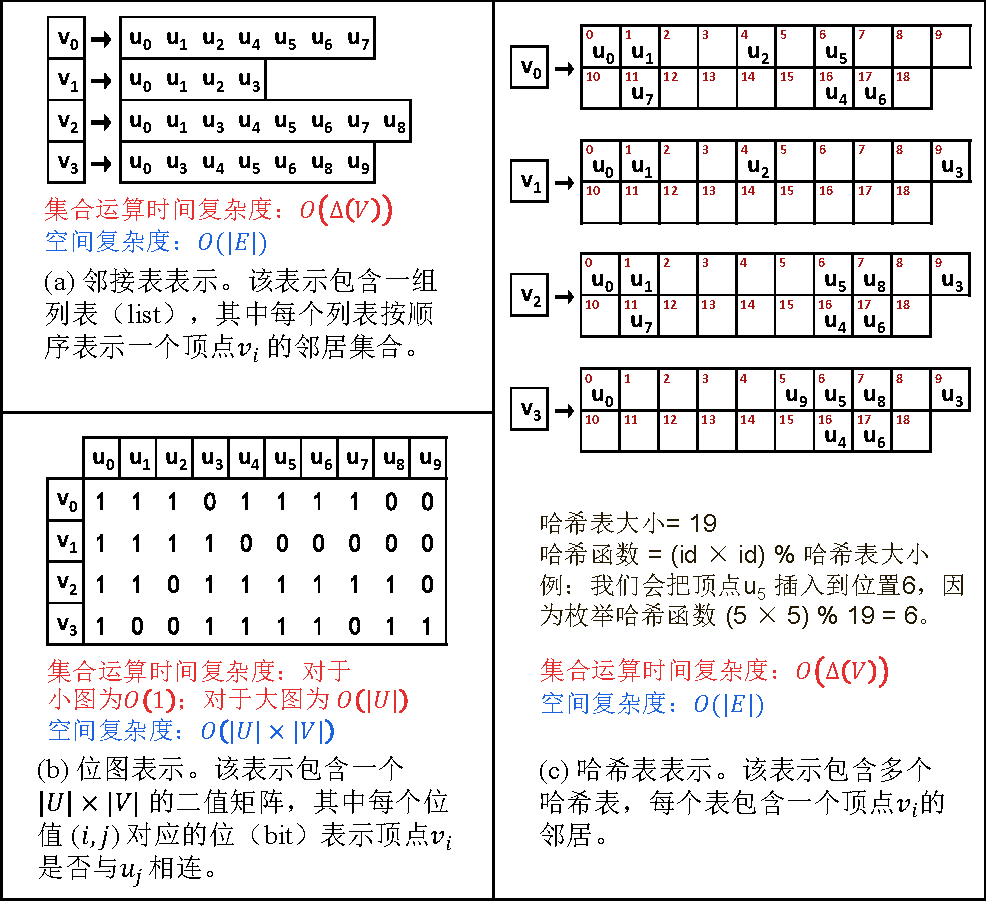
\includegraphics[width=0.9\linewidth]{adambe/eg_representation_full}
  \vspace{0.2in}
	\caption{二分图$G_2(U,V,E)$的三种存储结构}

	\label{fig:ada_graph_format}
\end{figure}

\textbf{邻接表。} 邻接表是一种常见的图存储结构,具有\emph{低存储使用}的优点,特别适用于稀疏图。在邻接表中,每个顶点都与一个包含其相邻顶点的链表相关联。这种存储结构节约内存,因为它只存储实际存在的边,而不需要额外的空间来存储缺失的边,因此它的空间开销仅为$O(|E|)$。此外,邻接表使得遍历图变得更加高效,因为我们可以通过遍历每个顶点的邻居链表来访问相邻顶点。邻接表在许多图算法中表现良好,特别是针对稀疏图的算法。然而,对于集合交集运算,邻接表可能会受到顶点度数较大的影响,因为每次交集操作都需要按顺序访问一个顶点的邻居,时间复杂度为$O(\Delta(V))$。在处理稠密图时,邻接表可能不如其他存储结构效率高,因为缺失的边在这类图中的占比较小,导致邻接表的低存储使用的优势无法凸显。邻接表存储结构广泛应用于最新的极大二分团枚举算法中,例如PMBE~\cite{PMBE20}和ooMBEA~\cite{ooMBE22}。

\textbf{位图。} 位图是另一种常见的图存储结构,在小图中具有\emph{计算高效}的特点,可以通过位运算实现集合交集运算,通常用于小图或密集图的存储。如图~\ref{fig:ada_graph_format}所示,在位图中,每个元素即一个位(bit),代表两个顶点的连接关系。与邻接表不同,位图在执行集合交集操作时不受顶点度数限制,因为它直接对应于所有可能的边。这使得位图在处理高度连通图时表现出色。在二分图中,通过两个$|U|$位位图之间的按位与操作(\&),可以计算出两个顶点的共同邻居,这个集合交集运算的时间复杂度为$O(|U|)$。对于小图,通过几次按位与操作,它可以在$O(1)$ 内高效地执行集合交集。然而,位图可能需要大量内存,特别是对于大型稀疏图,因为需要为所有缺失的边分配位。这可能会导致内存消耗过大,不适用于资源有限的情况。因此,位图存储结构仅应用于早期的基于小图的极大二分团枚举算法中,包括 LCM-MBC~\cite{lcmmbc07} 和 iMBEA~\cite{iMBEA14}。

\textbf{哈希表。} 哈希表是一种基于散列函数的数据结构,适用于\emph{快速查找和插入元素}的场景。在哈希表存储法下,二分图中每个顶点的邻居存放在一张哈希表中,每张哈希表通过哈希函数,能够在$O(1)$的时间内快速地查找某顶点是否在这张哈希表中。因此,在实现集合交集操作$A \cap B$时,假设集合$A$顶点数多于集合$B$的顶点数,我们可以通过将集合$B$中的每个元素分别在集合$A$对应的哈希表中进行查找的方式实现,因此集合交集运算的复杂度为$O(|B|)$。由此可知,哈希表在两个输入集合差异显著时,计算效果尤为明显。同时,部分完美哈希函数~\cite{cuckoohash04,murmurhash}能够实现空间复杂度与输入集合长度相同,因此得到与邻接表类似的空间复杂度。基于哈希表的存储结构,Jovan等人优化了极大团枚举算法的时间复杂度~\cite{MCE20}。然而,相比于邻接表,哈希表存储结构可能涉及大量的随机内存访问和更高的内存使用,效率不够理想。哈希表存储结构仅在 ParMBE~\cite{parMBE18} 中使用。


% 在图的表示中,哈希表通常用于某些特定的图算法。哈希表表示法通过高效的查找操作加速集合交集操作,尤其是在输入集大小差异显著时。虽然哈希表与邻接表具有类似的时间和空间复杂度,但可能涉及大量的随机内存访问和更高的内存使用。这可能导致性能相对较低,与邻接表相比效率不够理想。然而,在某些需要快速查找和动态更新的图算法中,哈希表表示法可能是更好的选择。哈希表表示法还可以处理图中的边属性信息,使得它在某些情况下更加灵活和实用。哈希表表示法仅在 ParMBE~\cite{parMBE18} 中使用。

\section{研究动机}

尽管已经有许多算法上的方法优化了极大二分团枚举问题的搜索空间,但是它们忽略了由数据结构限制带来的固有的计算低效性问题。这导致现有的算法只能应用于包含不超过1亿极大二分团的小数据集。因此,在本节中,我们将概括现有方法的数据结构限制,主要包括邻接表上进行集合运算的高计算开销以及算法中默认重复访问顶点的完整邻居带来的冗余计算。同时,我们将通过例子进行说明。为了方便表述,本章中默认以算法~\ref{alg:se_mbe} 在二分图$G_2$上的集合枚举树为例,如图~\ref{fig:ada_tree}所示。

\begin{figure} [t]
	\centering
  \vspace{0.1in}
	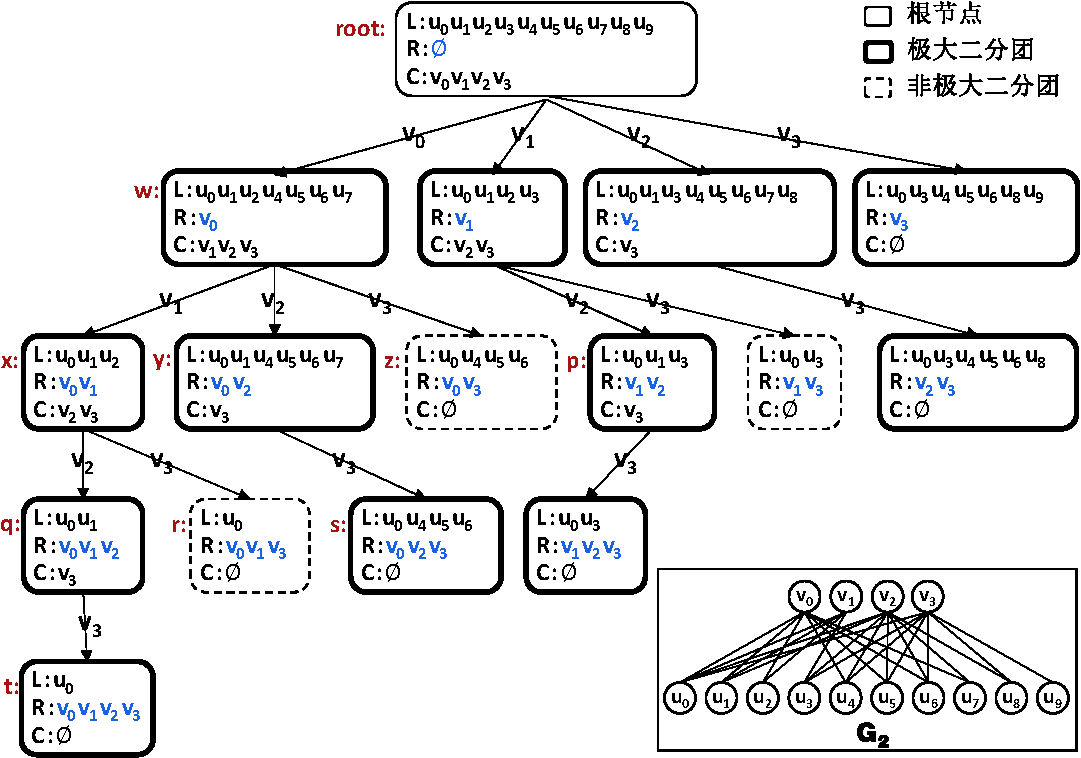
\includegraphics[width=0.9\linewidth]{adambe/eg_tree}
  \vspace{0.1in}
	\caption{算法~\ref{alg:se_mbe}在二分图$G_2$上的集合枚举树}

	\label{fig:ada_tree}
\end{figure}

\subsection{邻接表上的高集合运算开销}

\begin{table} [t]
	\centering    
	\setlength{\abovecaptionskip}{0.2cm}  
   \setlength{\belowcaptionskip}{0cm}
	\caption{MBE问题中集合运算时间以及冗余邻居访问占比}      
	\label{tbl:ada_motivation}
  \setlength{\tabcolsep}{2pt}
	\begin{center}
				\normalsize{
          \begin{tabularx}{0.95\linewidth}{|>{\centering\arraybackslash}X|*{12}{>{\centering\arraybackslash}p{0.75cm}|}}
            \hline
            \textbf{数据集} &\textbf{UL} & \textbf{UF} & \textbf{Mti} & \textbf{TM} & \textbf{AM} & \textbf{WC} & \textbf{YG} & \textbf{SO} & \textbf{Pa} & \textbf{IM} & \textbf{BX} & \textbf{GH}\\
            \hline
            \textbf{集合运算时间占比 \%} & 55.8&	52.6&	65.9&	31.5&	55.8&	38.1 & 70.0&	73.4&	35.7&	58.2&	76.4&	85.4\\
            \hline
            \textbf{冗余邻居访问占比 \%} & 89.6&	96.6&	96.7&	99.8&	95.9&	99.7 & 99.5&	99.5&	97.6&	97.4&	99.9&	98.9\\
            \hline
          \end{tabularx}
				}
	\end{center}

\end{table}


近年来,极大二分团枚举算法通常以邻接表作为存储二分图的首选方式。这主要是因为在处理大规模稀疏图的情况下,相比于其他图存储结构,邻接表结构具有最小的存储开销~\cite{PMBE20,ooMBE22}。然而,基于邻接表进行集合操作需要对两个集合对应的链表进行顺序串行比较,带来较大的计算开销。通过对基准算法MBEA~\cite{iMBEA14}在真实数据集中的实验统计,我们发现\emph{邻接表上的集合交集运算时间总是占据大部分的总运行时间}。表~\ref{tbl:ada_motivation}中的数据显示,在大多数数据集中,基于邻接表的集合交集运算耗时占据超过50\%的总运行时间,尤其在耗时最长的Github数据集上高达85.4\%。因此,优化基于邻接表的集合交集运算对于极大二分团枚举算法具有巨大的优化潜力。

具体而言,在图~\ref{fig:adambe_intersection} 中我们比较了邻接表与位图的集合运算实例。由于邻接表采用顺序连续存储的方式,进行集合操作通常需要串行访问和比较,导致操作时间与集合大小成正比,效率较低。相比之下,位图始终以等长方式存储顶点的所有邻居,因此每次集合操作可以通过固定长度的位运算(如与操作)实现。对于较小且密集的图情境,位图能够在常数时间内高效执行集合操作;然而,对于大规模稀疏图,由于其较高的内存需求,使用位图变得不切实际。因此,我们需要一种能平衡内存消耗和集合操作效率的自适应数据结构。


% 根据表~\ref{tbl:ada_motivation} 的数据,邻接表上的集合交集可能占据超过 50\% 的运行时间,这也是极大二分团枚举过程中主要的计算时间消耗部分,具有很高的优化潜力。

% 然而,表~\ref{tbl:ada_motivation} 表明,邻接表上的集合交集可能占据超过 50\% 的运行时间,主要是由于对顶点邻居的顺序访问所致。我们在图~\ref{fig:adambe_intersection} 中通过比较邻接表与位图的集合运算实例,对邻接表上的集合运算低效性进行进一步阐述。虽然位图表示能够通过位运算与操作(\&)实现高效的集合交集运算,但对于大型二分图来说,由于其高内存需求,变得不切实际。因此,需要一种平衡内存使用和集合运算时间的自适应的数据结构。



\begin{figure} [H]
	\centering
	\vspace{0.1in}
	\subfloat[邻接表]{
		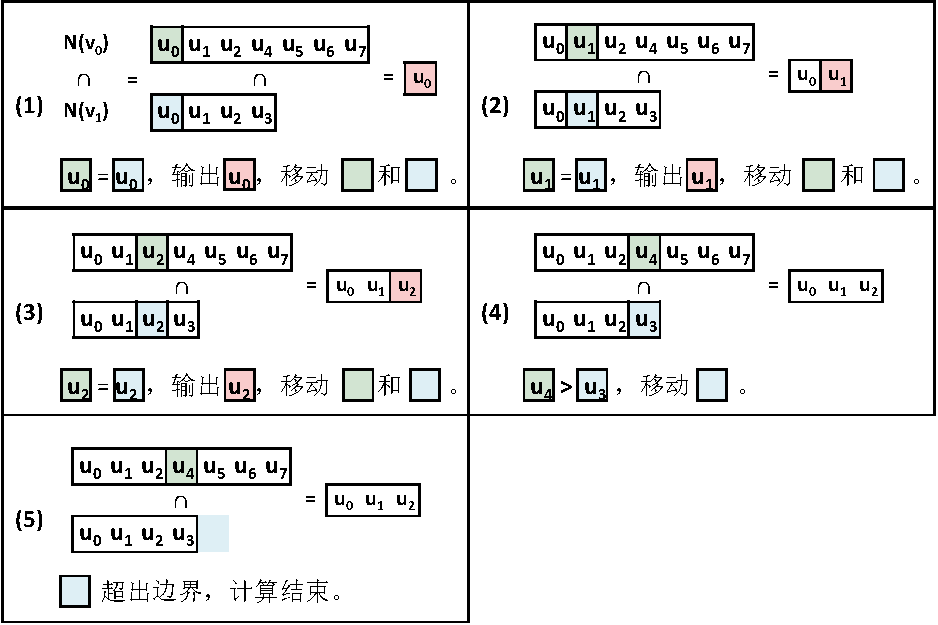
\includegraphics[width=0.85\linewidth]{adambe/eg_intersection_adjlist}
		\label{fig:adambe_intersection_adjlist}
	}
  \\
	\subfloat[位图]{
		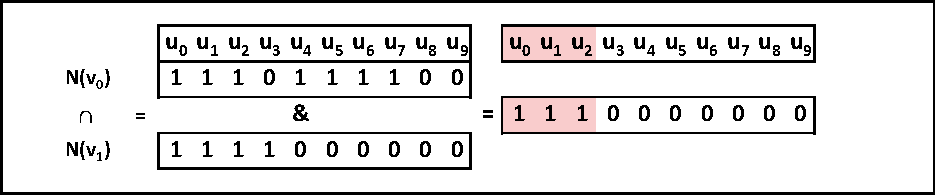
\includegraphics[width=0.85\linewidth]{adambe/eg_intersection_bitset}
		\label{fig:adambe_intersection_bitset}
	}
	\vspace{0.1in}
	\caption{邻接表与位图的集合交集运算比较实例$N(v_0)\cap N(v_1)$}
	
	\label{fig:adambe_intersection}
\end{figure}


\begin{example}
	
	在图~\ref{fig:adambe_intersection}中,展示了二分图$G_2$上$v_0$和$v_1$的共同邻居在邻接表和位图中的计算过程。图~\ref{fig:adambe_intersection_adjlist}则展示了一种基于邻接表的集合交集运算计算过程,采用双指针法。具体而言,首先,我们初始化两个指针,分别指向两个已排序集合的起始位置,并在集合中用绿色和蓝色标记指针位置。随后,我们不断地比较两个指针指向的元素。如果相等,则将该元素添加到交集中,并同时将两个指针向后移动一位(步骤\Num1、\Num2、\Num3);如果不相等,则将指向较小元素的指针向后移动一位(步骤\Num4)。最后,我们重复以上过程,直到其中一个集合的指针到达末尾为止(步骤\Num5)。除双指针法外,基于邻接表的集合运算方法还包括融合路径法~\cite{GpuMergePathIntersect14,MergePath18}、二分法~\cite{BinaryIntersect18,triangle18}等。然而,由于邻接表顺序连续存储的特性,集合运算至少需要对两个输入集合中的一个进行串行顺序访问。这意味着集合运算所需的时间与集合的大小直接相关,导致了较低的运算效率。
	
	图~\ref{fig:adambe_intersection_bitset}展示了一种基于位图的集合交集运算计算过程,采用位运算。具体来说,在二分图$G_2(U,V,E)$中,集合$V$中每个顶点$v$的邻居存储在一个长度为$|U|$的位图中,其中每一位代表$v$的邻居中是否存在对应元素。在位图存储下,我们通过对两个位图进行按位与(AND)操作,即可得到运算结果。因此,在$|U|$较小的情况下,由于位操作的计算复杂度较低,基于位图的集合交集运算更加高效。

\end{example}

% 图~\ref{fig:ada_motivation_2}展示了图~\ref{fig:ada_eg_tree}所示枚举树中父节点$w$和子节点$x$中涉及的部分集合交集运算。这些计算包括对每个节点的集合$L$以及对每个节点候选集合$C$的计算过程。

% 在每个节点的计算中,我们发现存在由无关顶点引起的冗余计算。除了我们提到的$L_x$的计算过程外,其他集合运算过程同样存在冗余。例如,在子节点$x$的集合$N_x(v_2)$的计算过程中,我们可以通过访问父节点中候选顶点$v_2$的局部邻居$N_w(v_2)$得到正确的计算结果,避免对$v_2$的全部邻居$N(v_2)$进行访问。因为根据推导$N_x(v_2) = L_x\cap N(v_2) = L_x \cap L_w \cap N(v_2) = L_x \cap N_w(v_2)$,我们知道$N(v_2)\setminus N_w(v_2)$中的顶点$u_3$和$u_8$不会对$N_x(v_2)$的计算结果产生影响,涉及冗余计算。同理,$N_x(v_3)$计算过程中的$u_3$,$u_8$和$u_9$也涉及冗余计算。




\subsection{完整邻居访问导致的冗余计算}
\label{subsec:ada_limitation}

目前,现有的极大二分团枚举算法在运行过程中默认访问顶点的完整邻居。然而,我们观察到两个现象:其一,每个节点需要计算候选顶点的局部邻居作为中间结果;其二,我们可以通过仅访问顶点的局部邻居而不是完整邻居来确保正确性。这里,顶点$v$在节点$x$中的\textbf{局部邻居}被定义为$N(v)$和$L_x$的交集,\textbf{在本章中被记作$N_x(v)$}。换言之,\emph{枚举过程中绝大部分的非局部邻居访问不会对最终的计算结果产生影响},顶点完整邻居的重复访问会带来冗余计算问题,影响计算性能。表~\ref{tbl:ada_motivation}中的数据显示,这种冗余在大多数真实数据集中占据超过90\%的顶点访问量,尤其是在耗时较长的BookCrossing数据集上高达99.9\%。此外,在第~\ref{subsec:ada_design_2}节中,我们还将探讨枚举节点和集合操作级别上的其他类型的冗余。

具体而言,在图~\ref{fig:ada_motivation_2}中我们展示了计算父节点$w$和子节点$x$中的集合交集运算实例。我们可以利用父节点$w$中的局部邻居$N_w(v_1)$而不是计算$N(v_1)$来推导出$L_x$。这一推导可以表示为$L_x = L_w \cap N(v_1) = L_w \cap (L_w \cap N(v_1)) = L_w \cap N_w(v_1)$。通过观察这一推导,我们发现在计算$L_x$时存在访问无效顶点的\textbf{冗余}。这些顶点存在于$N(v_1) \setminus N_w(v_1)$中,因为它们不会对$L_x$的最终结果产生贡献(例如$u_3$)。事实上,表~\ref{tbl:ada_motivation}显示这种冗余在大多数数据集中占据超过90\%的顶点访问量。此外,在第~\ref{subsec:ada_design_2}节中,我们还将探讨枚举节点和集合操作级别上的其他类型的冗余。






\begin{figure} [H]
	\centering
  % \vspace{0.05in}
	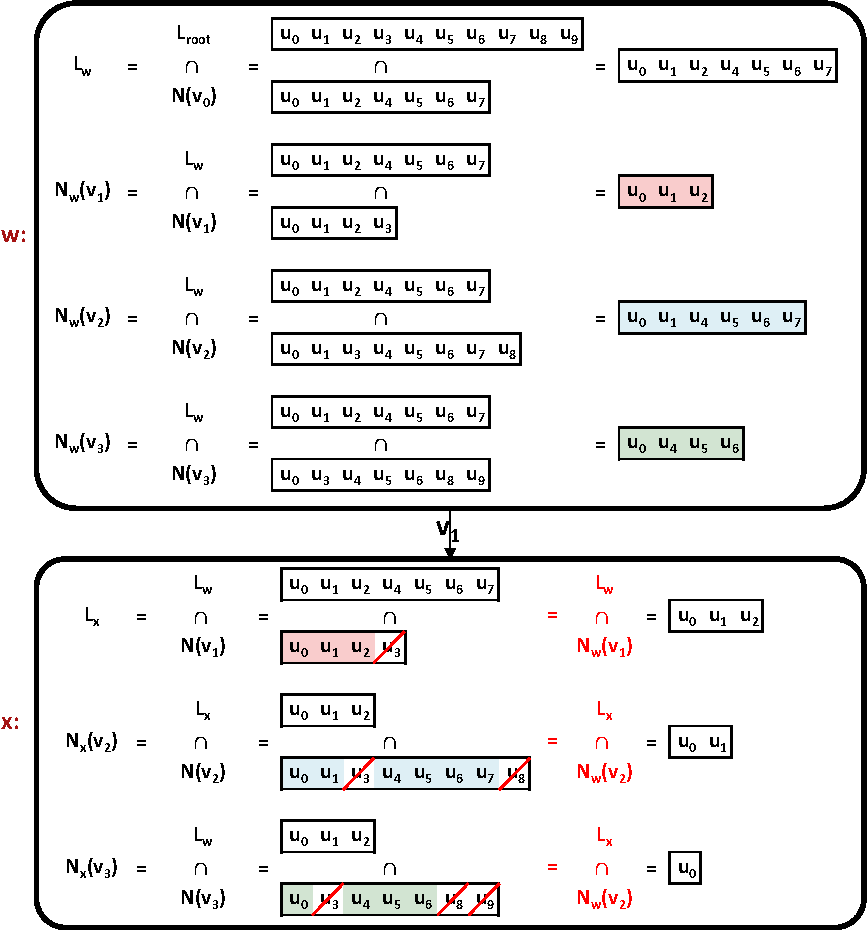
\includegraphics[width=0.85\linewidth]{adambe/eg_redundancy}
  % \vspace{0.05in}
	\caption{完整邻居访问导致的冗余计算示例}

	\label{fig:ada_motivation_2}

\end{figure}

\begin{example}
  图~\ref{fig:ada_motivation_2}展示了图~\ref{fig:ada_eg_tree}所示枚举树中父节点$w$和子节点$x$中涉及的部分集合交集运算。这些计算包括对每个节点的集合$L$以及对每个节点候选集合$C$的计算过程。

  在每个节点的计算中,我们发现存在由无关顶点引起的冗余计算。除了我们提到的$L_x$的计算过程外,其他集合运算过程同样存在冗余。例如,在子节点$x$的集合$N_x(v_2)$的计算过程中,我们可以通过访问父节点中候选顶点$v_2$的局部邻居$N_w(v_2)$得到正确的计算结果,避免对$v_2$的全部邻居$N(v_2)$进行访问。因为根据推导$N_x(v_2) = L_x\cap N(v_2) = L_x \cap L_w \cap N(v_2) = L_x \cap N_w(v_2)$,我们知道$N(v_2)\setminus N_w(v_2)$中的顶点$u_3$和$u_8$不会对$N_x(v_2)$的计算结果产生影响,涉及冗余计算。同理,$N_x(v_3)$计算过程中的$u_3$,$u_8$和$u_9$也涉及冗余计算。
  
\end{example}

\section{AdaMBE算法设计与实现}

为了克服现有方法的不足,本节提出了基于位图的动态子图方法和局部邻居缓存方法,以提升极大二分团枚举算法的效率。其中,基于位图的动态子图方法在枚举过程中动态创建子位图,并通过位运算加速了大量的集合运算;而局部邻居缓存方法通过动态缓存顶点的局部邻居,减少了枚举节点、集合运算以及顶点访问等三个层面的冗余计算。最终,我们综合应用这两种技术,形成了高效的自适应极大二分团枚举算法AdaMBE。

\subsection{基于位图的动态子图方法}
\label{subsec:ada_design_1}

为了优化邻接表上高昂的集合交集运算开销,我们提出了一种基于位图的动态子图方法,即BDS(bitmap-based dynamic subgraph)方法。不同于传统方法只采用单一的图存储方式,BDS方法融合了邻接表和位图两种图存储结构,利用邻接表表示整个二分图,在枚举过程中使用位图创建小型子图。通过这种方式,我们可以借助高效的位运算加速在极大二分团枚举过程中的集合交集运算。

BDS方法的设计基于我们的核心观察:\textbf{在枚举过程中,由活跃顶点诱导的计算图总是在不断缩小}。具体而言,在枚举过程中,根据算法~\ref{alg:se_mbe},新节点$(L',R',C')$中的集合$L'$和$C'$中的全部顶点均是源自父节点$(L, R, C)$对应的集合$L$和$C$(第4、8-9行),即$L'\subset L$且$C'\subset C$。由此可知,随着枚举过程的深入,节点内集合$L$和$C$中活跃顶点诱导的计算图也在不断缩小。因此,我们设计的BDS方法可以在当前节点对应的计算图大小小于我们给定的阈值时动态建立子位图,并充分发挥位图在高效集合交集运算方面的优势,在以当前节点为根节点的子枚举树中重用该子位图。

BDS方法的实现细节,我们通过回答以下两个关键问题的方式进行详细阐述:

\textit{(1)如何创建和利用基于位图的子图?}对于给定的节点$(L^*, R^*, C^*)$,我们利用位图从原始图$G(U, V, E)$中创建子图$G_{bitmap}(U',V',E')$。为了构建$U'$,我们选择了所有$L^*$中的顶点,因为$U \setminus L^*$中的顶点无法存在于$L'$中,也不会对算法~\ref{alg:se_mbe}(第4、6、8行)中的中间结果产生影响。为了构建$V'$,我们选择了不包括$R^*$内顶点在内的所有与$L^*$中任意顶点相连的顶点,存储为$\bigcup_{u \in L^*}N(u) - R^*$。这是因为未与$L^*$中任何顶点相连的顶点不能存在于$C'$ 或 $\Gamma(L')$中,也不能对算法~\ref{alg:se_mbe}中的中间结果产生影响。我们从$V'$中排除$R^*$中的顶点,因为它们总是出现在所有子节点的$R'$和$\Gamma(L')$中(第12行),这样可以减少冗余计算。$E'$包含原图内$U'$ 和$V'$之间的所有边。当 $U'$的大小(即$|L^*|$)小于某个给定的小的\emph{常数$\tau$}时,算法中的每个集合操作都可以通过按位与操作(\&)在$O(\tau) = O(1)$ 的时间内完成。我们通过检查对于所有$V'$中的顶点$v$是否满足$L' \cap N(v) = L'$来计算$\Gamma(L')$。这一节点检查过程需要$O(\tau \Delta(U))=O(\Delta(U))$ 的时间,因为$V'$最多包含$\tau \Delta(U)$ 个顶点,且每个顶点的集合交集运算只需 $O(1)$ 的时间。综上所述,创建和利用基于位图的子图使得能够加速极大二分团枚举算法中的集合运算过程,其中每个节点的计算时间为$O(\Delta(U))$。

\textit{(2)何时创建基于位图的子图? }为了优化集合交集操作并提高计算效率,在考虑当前节点 $(L^*, R^*, C^*)$的情况下,我们在满足以下条件时创建基于位图的子图:当$|L^*|$小于或等于阈值$\tau$且$C^*$ 不为空时。这些条件至关重要,因为$|L^*|$直接影响集合交集所需的时间,而$C^*$ 影响位图在子节点中的重用次数。然而,选择适当的阈值$\tau$是具有挑战性的。较大的$\tau$会增加集合交集的时间(即$O(\tau)$)和每个子图的内存使用。相反,较小的$\tau$会导致创建更多小的子图,从而限制了在子节点中位图的重用机会。因此,在确定$\tau$时,我们必须在集合交集计算的效率和位图的利用之间取得平衡。根据我们在第~\ref{subsec:ada_eval_sensitivity}节的实验,我们建议将阈值$\tau$设为64,因为这种情况下每次操作只需要对两个64位长长整数进行高效的按位与操作。

接下来,我们用一个实例进行说明:

\begin{figure} [H]
	\centering
  \vspace{0.05in}
	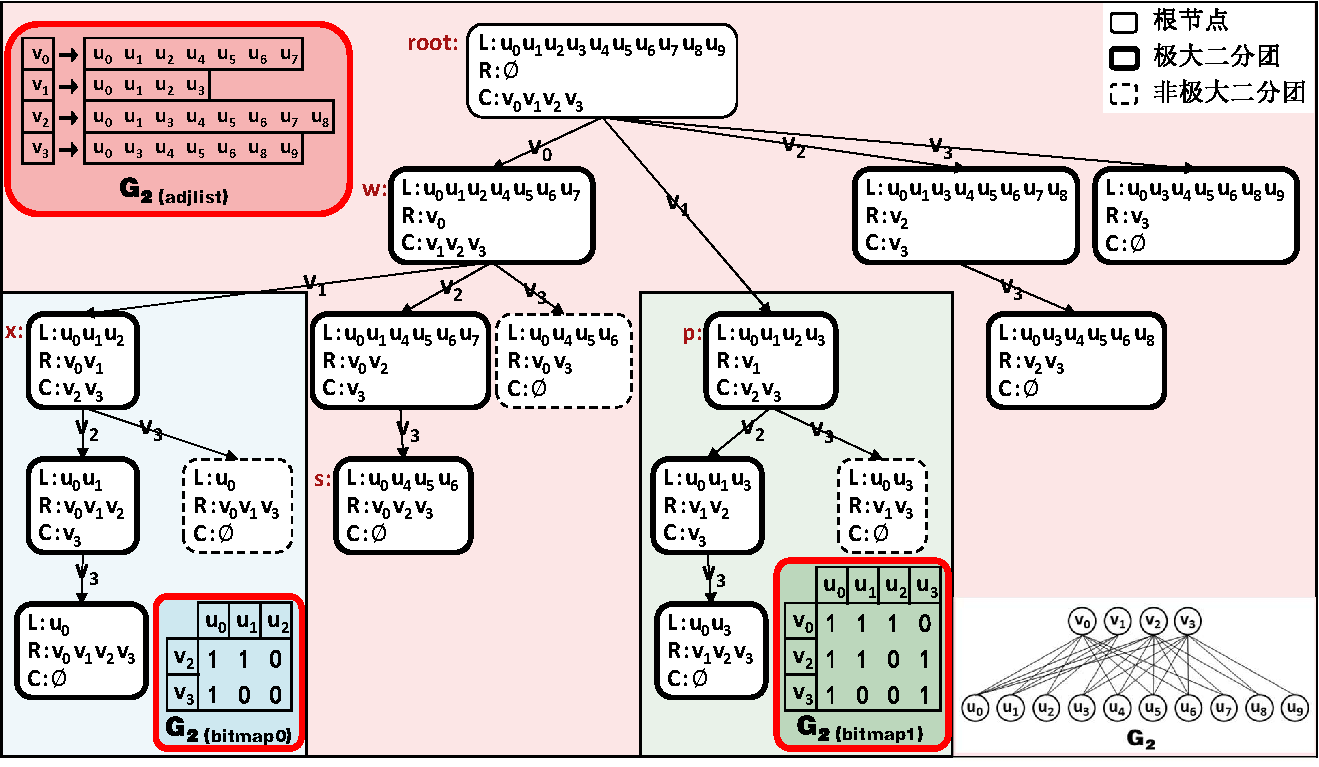
\includegraphics[width=\linewidth]{adambe/eg_design_1}
  \vspace{0.02in}
	\caption{基于位图的动态子图方法示例}

	\label{fig:ada_design1}
\end{figure}

\begin{example}
  图~\ref{fig:ada_design1}中展示了在二分图$G_2$上应用BDS方法进行极大二分团枚举的过程。在这个例子中,阈值$\tau$设置为4。最初,图$G_2$使用邻接表作为默认方法存储(标记为$G_{2(邻接表)}$)。当我们进入节点$x$时,我们观察到$|L_x| = 3 < \tau$,因此创建了基于位图的子图$G_{2(位图0)}$。在$G_{2(位图0)}(U_0, V_0, E_0)$中,$U_0$包含$L_x$中的所有顶点,即$u_0$,$u_1$和$u_2$。$V_0$包含$v_2$和 $v_3$,因为它们与$L_x$中的某些顶点有连接。$v_0$和$v_1$不属于$V_0$,因为它们属于$R_x$。因此,节点$x$的所有子节点都可以通过利用$G_{2(位图0)}$中的位图加快集合交集。类似地,在节点$p$处,我们创建另一个基于位图的子图$G_{2(位图1)}$,使得$p$节点的所有子节点都受益。尽管$|L_s| = 4 = \tau$,但我们避免在节点$s$处创建子图,因为$C_s$为空,这意味着如果此位图被创建,将没有子节点可以重用此位图。
  
\end{example}

  BDS方法的主要贡献包括以下两点:


  \begin{enumerate}
    \item \textbf{结合两种不同图存储结构的优势。} 在选择图的存储结构时,我们需要在计算效率和内存效率之间取得平衡。针对大型图,我们采用邻接表存储结构,因为它具有较好的内存效率;而对于小型子图,则使用位图存储结构,因为它具有较好的计算效率。我们的BDS方法在原始图和较大的子图上继续沿用邻接表存储,有效地控制了在极大二分团枚举过程中的内存使用。早期的极大二分团枚举算法研究在小型图$G(U, V, E)$上使用了位图存储~\cite{lcmmbc07,iMBEA14}。然而,即使在这些小型图中,如果$U$内的顶点数量不足够小,每次按位集合交集操作的时间复杂度仍为$O(|U|)$,而非$O(1)$。因此,在许多情况下,直接采用位图存储方式未必能达到理想的计算效率。相反,BDS方法通过设置一个小的阈值$\tau$限制$U$的大小,保证每次集合操作的完成时间为$O(1)$,从而保证了计算效率。
    
    \item \textbf{充分利用二分图的特点。} 相较于通用图,基于位图的子图技术特别适用于二分图。具体而言,对于只有一个顶点集$V$的通用图$G(V,E)$,我们很难确定何时创建位图。如果通用图顶点数$|V|$很大且稀疏,创建位图会导致内存使用效率低下。相反,如果$|V|$很小,则位图无法得到充分重用。最近的研究~\cite{Graphset23}指出,基于位图的子图优化在少数几项工作中受到限制~\cite{Sandslash21,Kclique22,g2miner22}。幸运的是,对于具有两个不相交顶点集$U$ 和$V$的二分图$G(U,V,E)$,我们可以通过小的$|U|$实现高效的内存使用,并通过大的$|V|$实现位图的有效利用。因此,BDS方法通过有效利用二分图的独特特性显著改进了极大二分团枚举问题。
  
  \end{enumerate}



\subsection{局部邻居缓存方法}
\label{subsec:ada_design_2}


为了减少因访问顶点的完整邻居而产生的冗余,我们提出了一种局部邻居缓存方法,即LNC(local neighbor caching)方法。其核心设计思想是动态缓存候选顶点的局部邻居,并重新利用这些中间结果,以避免对非活跃邻居进行大量内存访问。该方法有效地减少了三种类型的冗余:

(1) \emph{\textit{粗粒度冗余。}}
这种冗余指的是对应非极大二分团的\textbf{节点},如图~\ref{fig:ada_eg_tree} 所示的节点$z$和节点$r$。最近的极大二分团枚举算法优化工作侧重于裁剪这些节点以减少此类冗余~\cite{iMBEA14,PMBE20,ooMBE22}。LNC 方法为这些努力提供了补充。

(2) \emph{\textit{中等粒度冗余。}}
这种冗余源于枚举过程中重复的\textbf{集合}交集运算。从算法~\ref{alg:se_mbe} 中可以观察到,当父节点$p$遍历顶点$v_c$生成子节点$c$时,节点$p$中计算$v_c$局部邻居的过程始终与节点$c$中计算集合$L_c$的过程相同,即$L_p\cap N(v_c)$。例如,图~\ref{fig:ada_motivation_2}显示父节点 $w$使用$L_w\cap N(v_1)$计算$N_w(v_1)$,同时子节点$x$也使用$L_w\cap N(v_1)$计算$L_x$,这两个计算过程完全相同,存在冗余。尽管这种冗余在现有的极大二分团枚举算法中普遍存在,但没有算法试图解决这个问题。

(3) \emph{\textit{细粒度冗余。}}
这种冗余是指非活跃\textbf{顶点}的内存访问,即不是候选顶点的局部邻居的顶点。~\ref{subsec:ada_limitation} 节详细介绍了这个问题。其中表~\ref{tbl:ada_motivation} 表显示超过 90\% 的内存访问涉及这些无用的顶点。然而,现有工作忽视了这个重要的限制。

LNC方法通过缓存并利用候选顶点的局部邻居来实现。接下来,我们将通过解决三种冗余问题的方式进行详细阐述具体的实现细节:

(1) 为了减少由非极大二分团对应节点带来的粗粒度冗余,我们利用局部邻居这一中间结果进行剪枝。具体而言,当同一候选顶点$v$的局部邻居在父节点$p$和子节点$c$中保持不变时,我们可以安全的裁剪掉由节点$p$遍历顶点$v$生成的节点。这是因为根据极大二分团枚举算法深度优先搜索的策略,父节点将会产生一个非极大二分团。关于这一点,我们将在第~\ref{subsec:gmbe_prune}节中的定理~\ref{theorem:gmbe_prune}处进行详细描述。在这种情况下,我们将 $N_p(v)$和$N_c(v)$存储在相同的内存空间中,以减少内存使用,因为它们是相同的。

(2)为了避免由重复集合交集引起的中等粒度冗余,我们将每个候选顶点的局部邻居存储在它们各自的子节点中。当父节点$p$遍历候选顶点$v$生成子节点$c$时,子节点$c$可以直接访问$L_c$而无需进行冗余计算,因为$L_c$始终等同于预先存储的局部邻居 $N_c(v)$。

(3)为了避免由于非活动顶点的内存访问而导致的细粒度冗余,我们决定对所有局部邻居进行缓存。这样一来,我们可以只访问顶点的必要局部邻居,而不是整个邻居集合。具体而言,子节点$c$ 可以通过使用父节点$p$缓存的局部邻居来计算每个$C_c$ 中的顶点$v$ 的局部邻居。这一计算过程可以表达为$N_c(v) = L_c \cap N(v) = L_c \cap (L_p \cap N(v)) = L_c \cap N_p(v)$,其中$L_c$ 总是$L_p$的子集。这一设计可使我们更高效地利用已经计算过的中间结果,从而进一步减少内存访问和计算量。

接下来,我们用一个实例进行说明:

\begin{figure} [H]
	\centering
  \vspace{0.05in}
	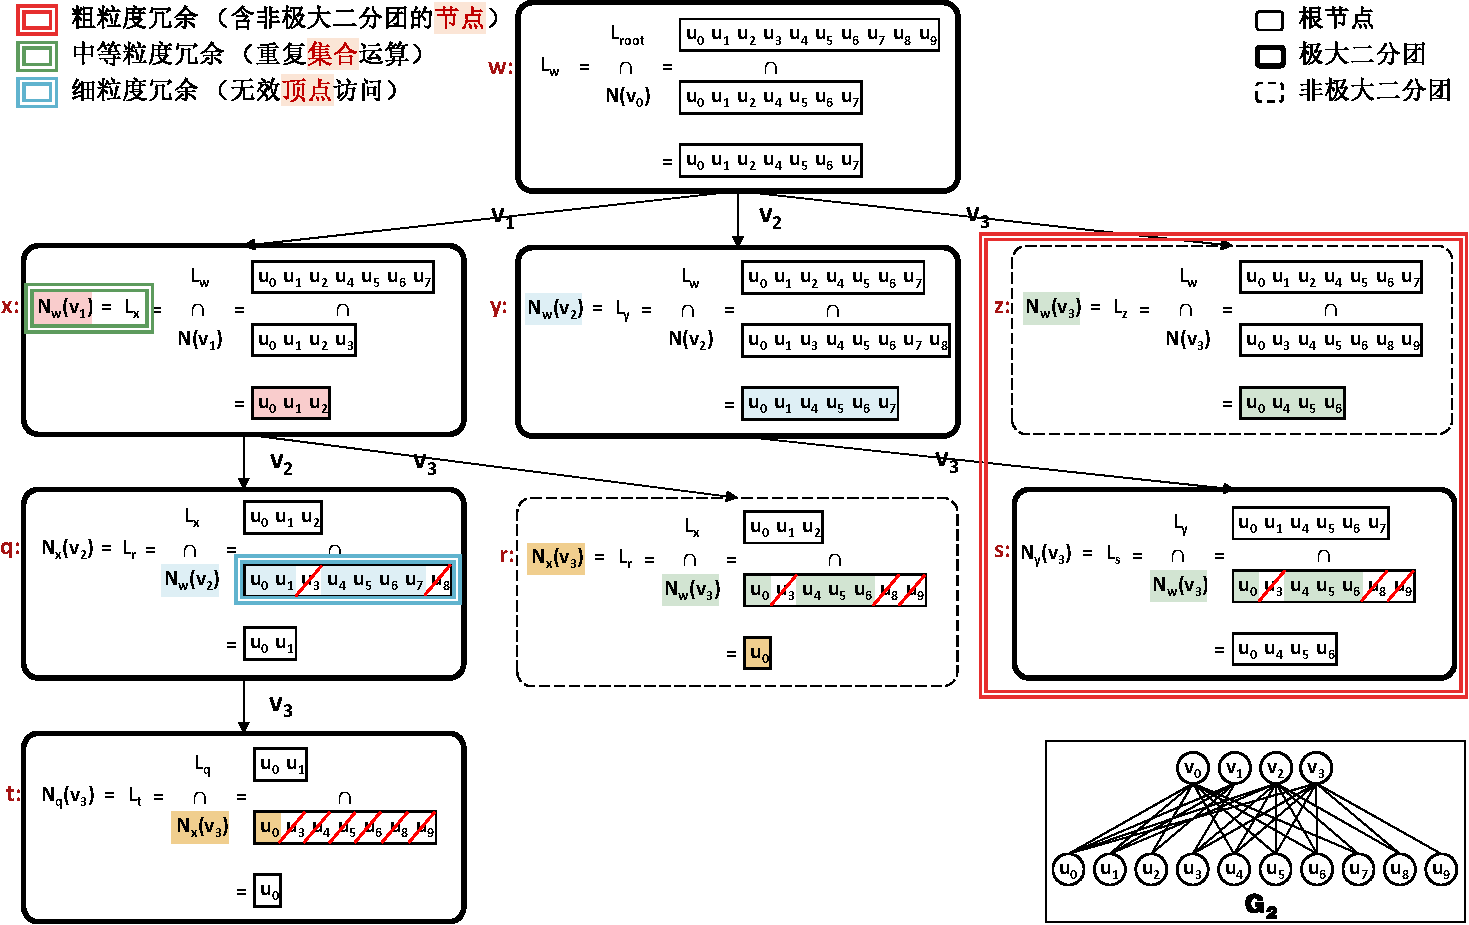
\includegraphics[width=\linewidth]{adambe/eg_design_2}
  % \vspace{0.05in}
	\caption{局部邻居缓存方法示例}

	\label{fig:ada_design2}
\end{figure}

\begin{example}
  图~\ref{fig:ada_design2} 中展示了以图~\ref{fig:ada_eg_tree} 中节点 $w$ 为根的子树中使用 LNC 方法的过程。我们根据局部邻居大小进行裁剪,去除非极大二分团的节点(粗粒度冗余)。例如,节点 $w$ 将其子节点 $z$ 进行裁剪,因为节点 $w$ 知道当前遍历顶点 $v_3$ 的局部邻居大小保持不变,即 $|N_w(v_3)| = |N_y(v_3)| = 4$。我们通过在子节点中存储候选顶点的局部邻居来避免重复的集合交集操作(中等粒度冗余)。例如,节点 $w$ 在其子节点 $x$、$y$ 和 $z$ 中分别存储局部邻居 $N_w(v_1)$、$N_w(v_2)$ 和 $N_w(v_3)$。这样每个节点就可以直接使用缓存的局部邻居访问其集合$L$,比如节点 $x$ 可以将 $L_x$ 访问为 $N_w(v_1)=L_x$。我们通过仅利用缓存的局部邻居而非完整邻居来最小化内存访问(细粒度冗余)。例如,节点 $q$ 使用局部邻居 $N_w(v_2)$ 来计算 $N_x(v_2)$,而非完整邻居 $N(v_2)$。这一方法避免了访问不相关顶点,如 $u_3$ 和 $u_8$。
\end{example}

LNC方法的主要贡献包括以下两点:

\begin{enumerate}
  \item \textbf{提升中间结果的利用率。} 在现有的极大二分团枚举算法中,局部邻居是必要的中间结果。LNC方法通过缓存这些中间结果来优化它们的使用。通过利用父节点和子节点之间的关系,在节点计算过程中我们将完整邻居替换为局部邻居。虽然需要额外的内存来存储局部邻居,但是这种方法平均减少了非活跃顶点的内存访问量达到了97.1\%,从而提高了效率,具体数据已在~\ref{subsec:ada_limitation} 节中展示。考虑到内存不是计算密集型的极大二分团枚举问题的瓶颈,为了减少运行时间而交换内存空间是值得的。

\item \textbf{同时解决多种类型的冗余。} 在缓存局部邻居之后,我们识别出了枚举过程中存在的三种冗余类型。与传统方法只考虑节点层面冗余不同,我们还解决了在集合操作和顶点访问层面上存在的隐藏冗余。通过精心调整局部邻居以分别处理这些冗余,我们取得了出色的整体性能。在整个图挖掘领域,最新算法开始注意到重复集合运算带来的冗余~\cite{Graphpi20,GPMredundancy23},即我们定义的中等粒度冗余。然而,与这些已有方法相比,LNC方法额外关注了顶点层面更细粒度的冗余,并进行了解决。

\end{enumerate}

\subsection{AdaMBE算法}

结合BDS方法和LNC方法,我们设计了一种自适应的极大二分团枚举算法,简称为AdaMBE(adaptive maximal biclique  enumeration)。该算法的基本思想是在极大二分团枚举过程的不同阶段分别应用这两种方法,即使用BDS方法处理基于小图的子位图,使用LNC方法处理基于原图的邻接表。这是因为在小图场景下,BDS方法可以通过位运算提升集合交集运算的效率,在处理小图时性能优于LNC方法;而在大原始图的场景下,LNC方法有效填补了BDS方法没有优化的空白。此外,对于一个二分图$G(U,V,E)$,AdaMBE会根据它们的邻居大小对集合$V$中的所有顶点进行初始排序,我们将在~\ref{subsec:ada_eval_sensitivity} 节通过实验展示其高效性。

接下来,我们从时间复杂度和空间复杂度两个方面对AdaMBE进行讨论。

\textbf{时间复杂度:} 与第~\ref{ch:aggressive_mbe}章介绍的AMBEA算法相似,AdaMBE算法的时间复杂度由顶点排序时间和集合枚举树生成时间组成。其中,按照顶点度数升序排列的时间复杂度为$O(|V|log(|V|))$,在邻接表中每个节点的计算时间为$O(|E|)$,而在位图中每个节点的计算时间为$O(\Delta(U))$。为了量化算法的计算时间,我们将$\beta$用于表示枚举树中节点的数量,包括输出极大二分团的节点和产生非极大二分团的节点。这里,我们将$\beta$分解为两部分,即$\beta_0$表示基于邻接表计算的枚举节点,而$\beta_1$表示基于子位图计算的枚举节点。最终,我们得到AdaMBE的计算复杂度为$O(|E|\beta_0 + \Delta(U)\beta_1 + |V|log(|V|))$。由于排序开销通常远小于生成集合枚举树的开销,因此,AdaMBE的时间复杂度可以简化为$O(|E|\beta_0 + \Delta(U)\beta_1 )$。在~\ref{subsec:ada_breakdown} 节的细分评估实验中,我们观察到在真实数据集中,$\beta_1$通常占据了大部分的计算时间,因此相较于其他算法,AdaMBE表现出明显的性能提升。

\textbf{空间复杂度:} AdaMBE算法的空间复杂度可分为两部分:输入二分图所需空间和极大二分团枚举过程的空间。输入二分图所占用的空间为$O(|E|)$。在枚举过程中,LNC方法会动态保存顶点的局部邻居,构成原二分图的一个子图,因此每个节点所需空间为$O(|E|)$。由于枚举树的高度上限为$O(\Delta(V))$,因此AdaMBE的空间复杂度为$O(|E|+|E|\Delta(V)) = O(|E|\Delta(V))$,略高于当前最优算法的空间复杂度$O(|E|+|V|\Delta(V))$。这是因为AdaMBE算法中的LNC方法需要额外空间以增加局部邻居的重用性,从而提升计算性能。在~\ref{subsec:ada_overall} 节的整体评估实验中,我们观察到在测试的真实数据集上,AdaMBE的最大内存使用仅约为1GB,并且在大多数情况下,AdaMBE算法的内存占用仍低于先进算法PMBE和ooMBEA,因此相对于LNC方法带来的计算性能提升,其空间开销是可以接受的。

\textbf{并行扩展:} 为了进一步提升性能,我们在AdaMBE算法的基础上设计了其并行版本ParAdaMBE。受到并行算法ParMBE~\cite{parMBE18}的启发,ParAdaMBE利用Intel TBB库~\cite{tbb-code}的功能,为二分图集合$V$中的每个顶点$v$分配一个线程,负责处理由顶点$v$产生的子枚举树。这样,多个枚举树可以无重叠地并发计算。此外,只要存在额外线程可用,ParAdaMBE将对子枚举树对应的任务进行进一步分解。为了进一步提升并行计算资源的利用,ParAdaMBE通过循环展开技术有效并行化算法中的for循环,最大程度地利用并行性缩短算法的运行时间。

与现有的极大二分团枚举方法专注于算法搜索空间优化不同,AdaMBE强调数据结构的优化。它根据处理图的大小灵活选择BDS和LNC技术,优化了极大二分团枚举过程中最耗时的集合运算过程,显著改善了计算效率。此外,BDS技术中的邻接表与位图混合存储方法以及LNC技术中的局部邻居缓存方法具有通用性,能够为其他图挖掘算法的数据结构优化提供思路,为图分析领域提供可行的技术路径。











\section{实验评估}

\subsection{实验设置}

\textbf{实验环境设置:} 本节的全部实验均在一台配备有4个Intel Xeon(R) Gold 5318Y 2.10GHz CPU和128GB内存的服务器上完成,其中每个CPU拥有24个计算核心,共计96个计算核心。本次实验环境的操作系统为Linux kernel-5.4.0。在没有特殊说明的情况下,算法默认使用单个计算核心串行执行。鉴于现有算法在大规模数据集上很难在短时间内完成,我们将运行时间限制设置为48小时(INF)。

\textbf{比较算法:} 在我们的实验中,我们评估了串行和并行极大二分团枚举算法的性能。对于串行算法,我们将AdaMBE与过去五年中的三种最先进的算法进行了比较:FMBE~\cite{parMBE18},PMBE~\cite{PMBE20} 和 ooMBEA~\cite{ooMBE22}。对于并行算法,我们将 ParAdaMBE 与目前最先进的多线程并行算法ParMBE~\cite{parMBE18}进行比较。默认情况下,我们在同一台拥有 96 个核心的 CPU 的服务器上使用 96 个线程来运行ParAdaMBE和ParMBE。此外,为了深入评估本章提到的技术点,我们实现了一些算法变体,并在对应实验中详细描述。

\begin{table} [t]
	\centering    
	\setlength{\abovecaptionskip}{0cm}  
  \setlength{\belowcaptionskip}{-0.2cm}
	\caption{AdaMBE增加的实验数据集统计信息}      
	\label{tbl:ada_datasets}
	\setlength{\tabcolsep}{1pt}
	\begin{center}
				\normalsize{
		\begin{tabular}{|c|c|c|c|c|c|c|}
			\hline 
			\textbf{数据集} &\textbf{目录} &\textbf{类型} & \textbf{$|U(G)|$} & \textbf{$|V(G)|$} & \textbf{$|E(G)|$} &\textbf{极大二分团}\\
			\hline
			% Unicode (UL) & 特征关系 & 国家-使用-语言 &  614 & 254 & 1,255 & 460\\
			% UCforum (UF) & 交互关系 & 用户-发布-论坛 & 899 & 522 & 7,089 & 16,261\\
			% % Wikinews & 作者关系  & 用户-编辑-文章 & 41,747  & 1,572 & 109,218 & 44,444\\
			% %Writers (WR) & 作者关系 & 作者-出版-作品 & 89,355 & 46,213 & 144,340 & 57,222\\ 
			% MovieLens (Mti) & 特征关系 & 标签-属于-电影 & 16,528 & 7,601 & 71,154 & 140,266\\ 
			% Teams (TM) & 归属关系 & 队员-属于-团队 & 901,130 & 34,461 & 1,366,466 & 517,943 \\
			% ActorMovies (AM) & 归属关系 & 电影-出演-演员 & 383,640 & 127,823 & 1,470,404 & 1,075,444\\ 
			% Wikipedia (WC) & 特征关系 & 文章-属于-目录 &1,853,493 & 182,947 & 3,795,796 & 1,677,522 \\
      % YouTube (YG) & 归属关系 & 用户-属于-群组 & 94,238 & 30,087 & 293,360 & 1,826,587\\  
			% StackOverflow (SO) & 评分关系 & 作者-收藏-帖子 & 545,195 & 96,680 & 1,301,942 & 3,320,824 \\
			% DBLP (Pa) & 作者关系 & 作者-出版-作品 & 5,624,219 & 1,953,085 & 12,282,059 & 4,899,032\\
			% IMDB (IM) & 归属关系 & 电影-出演-演员 & 896,302 & 303,617 & 3,782,463 & 5,160,061\\
			% BookCrossing (BX) & 交互关系 & 用户-打分-书籍  & 340,523 & 105,278 & 1,149,739 & 54,458,953 \\
			% Github (GH) & 作者关系 & 用户-参与-工程 & 120,867 & 56,519 & 440,237 & 55,346,398 \\ 
      CebWiki (ceb) & 作者关系 & 用户-编辑-文章 & 8,483,068 & 3,132 & 11,792,890 & 263,138,916\\
			TVTropes (DBT) & 特征关系 & 作品-拥有-特征 & 87,678 & 64,415 & 3,232,134 & 19,636,996,096 \\ 
      \hline
      LJ10 & 归属关系 & 用户-属于-群组& 2,301,031& 1,421,088& 11,227,130& 7,430,705\\
			LJ20 & 归属关系 & 用户-属于-群组& 2,704,651& 2,357,485& 22,456,757& 61,836,924\\
			LJ30 & 归属关系 & 用户-属于-群组& 3,163,966& 2,889,804& 33,686,334& 343,257,225\\
			LJ40 & 归属关系 & 用户-属于-群组& 3,894,262& 2,992,774& 44,917,368& 1,524,229,722\\
			LJ50 & 归属关系 & 用户-属于-群组& 4,572,628& 3,057,410& 56,150,150& 6,387,845,280\\
      
      % \hline
			% LJ5 & 归属关系 & 用户-属于-群组& 1,837,928 & 853,994 & 5,610,437 & 2,181,295 \\
			% LJ10 & 归属关系 & 用户-属于-群组& 2,301,031 & 1,421,088 & 11,227,130 & 7,430,705 \\
			% LJ15 & 归属关系 & 用户-属于-群组& 2,548,619 & 1,912,139 & 16,843,216 & 22,727,251 \\
			% LJ20 & 归属关系 & 用户-属于-群组& 2,704,651 & 2,357,485 & 22,456,757 & 61,836,924 \\
			% LJ25 & 归属关系 & 用户-属于-群组& 2,812,080 & 2,771,510 & 28,068,423 & 151,468,807 \\

			% LiveJournal & 归属关系 & 用户-属于-群组 & 7,489,073 & 3,201,203 & 112,307,385 & -\\
			% WebTrackers & Hyperlink & Domain-Inclusion-Tracker & 27,665,730 & 12,756,244 & 140,613,762 & -\\ 
			\hline
		\end{tabular}
				}
	\end{center}
	\vspace{-0.1in}
\end{table}



\textbf{数据集:} 为了准确评估本章提出的技术,我们同时使用了真实数据集和合成数据集。为了进一步探索 AdaMBE 在包含超过 1 亿极大二分团的大数据集上的性能,我们在上一章实验中的表~\ref{tbl:datasets} 的基础上额外增加了大数据集,如表~\ref{tbl:ada_datasets} 所示。其中,真实数据集 CebWiki 和 TVTropes 来源于 KONECT 仓库~\cite{konect},TVTropes数据集包含的极大二分团数量超过了196亿。合成数据集是在大数据集 LiveJournal ($|U|$=7,489,073, $|V|$=3,201,203, $|E|$=112,307,385) 上分别采样 10\%、20\%、30\%、40\% 和 50\% 的边所生成,分别记作 LJ10、LJ20、LJ30、LJ40 和 LJ50。大数据集 LiveJournal 也来自于 KONECT 仓库。

\subsection{整体评估}
\label{subsec:ada_overall}

\textbf{常规数据集上的性能评估:} 为了验证我们提出的算法的整体效率,我们在12个常规数据集上测量了所有竞争对手的运行时间和内存使用情况。运行时间不包括从磁盘加载图的时间,内存使用表示相应进程的最大内存占用。


\begin{figure} [H]
  \centering
  \subfloat[运行时间 (对数形式)]{
		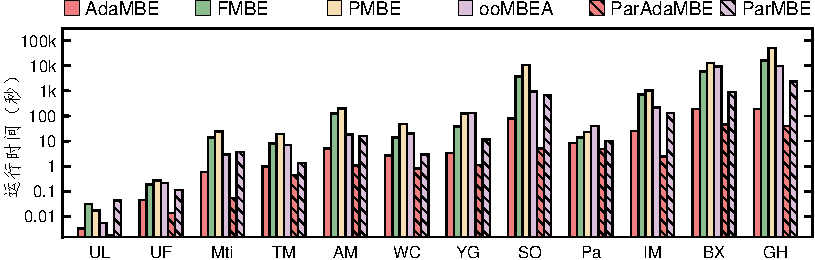
\includegraphics[width=0.95\linewidth]{adambe/overall_time}
		\label{fig:ada_overall_time}
	}
	\vspace{0.1in}
	\\
  \subfloat[内存使用(对数形式)]{
		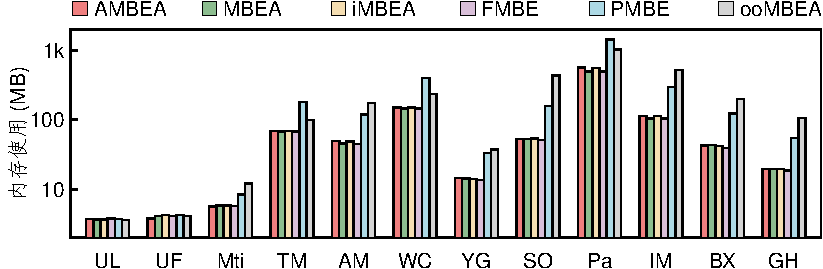
\includegraphics[width=0.95\linewidth]{adambe/overall_memory}
		\label{fig:ada_overall_memory}
	}
  \caption{AdaMBE在常规数据集上的整体评估}
  \label{fig:ada_overall}

\end{figure}

图~\ref{fig:ada_overall_time} 显示,不同数据集下,我们的串行算法 AdaMBE 始终比其最接近的串行竞争对手快 1.6-49.7倍,而我们的并行算法 ParAdaMBE 始终比 ParMBE算法快2.5-137.8倍。得注意的是,在耗时最长的数据集 Github 上,AdaMBE 在 194 秒内完成任务,而其他串行竞争对手则需要超过 9,638 秒。类似地,ParAdaMBE 在 40 秒内完成,而ParMBE需要超过 2,412 秒。

图~\ref{fig:ada_overall_memory} 显示,与同类别中的其他算法相比,我们串行和并行算法的内存使用情况类似。尽管我们的算法 AdaMBE 需要额外的内存来存储局部邻居,但它仍然优于最近的串行算法 PMBE 和 ooMBEA。事实上,PMBE 和 ooMBEA 分别需要比 AdaMBE多1.4倍和1.9倍的内存,因为它们需要额外的内存来存储 CDAG 索引结构~\cite{PMBE20} 和多个子图~\cite{ooMBE22}。


\begin{figure} [H]
  \centering
  \subfloat[CebWiki数据集上的运行时间评估
		% Evaluation on CebWiki. We report running time of all competitors excluding GMBE, which runs out of memory (OOM).
		]{
		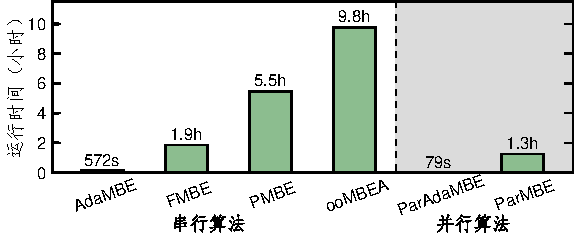
\includegraphics[width=0.8\linewidth]{adambe/cebwiki}
		\label{fig:ada_overall_cebwiki}
	}
	\\
  \subfloat[TVTropes数据集上48小时内算法输出的极大二分团数量
		% Evaluation on TVTropes. As only AdaMBE and \parpname{} complete within 48 hours, we report the maximal biclique count of competitors at 48 hours.
		]{
		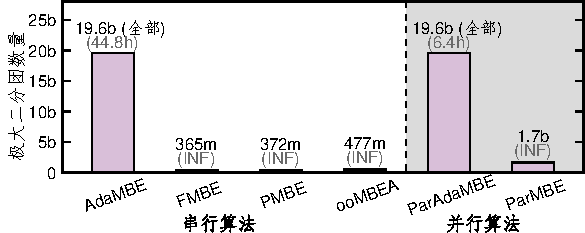
\includegraphics[width=0.8\linewidth]{adambe/tvtropes}
		\label{fig:ada_overall_tvtropes}
	}

  \caption{AdaMBE在超大数据集上的整体评估}
  \label{fig:ada_overall_large}
\end{figure}


\textbf{大规模数据集的评估:} 我们进一步在包含超过2亿个极大二分团的大型数据集上评估我们的算法。图~\ref{fig:ada_overall_cebwiki} 显示,所有其他竞争对手在 CebWiki 数据集上完成 MBE 需要数小时,而我们的 AdaMBE 和 ParAdaMBE 仅分别需要 572 秒和 79 秒。由于没有现有竞争对手能在包含190亿个极大二分团的 TVTropes 数据集上完成枚举,我们报告了所有算法在48小时内的极大二分团数量。图~\ref{fig:ada_overall_tvtropes} 显示,其他竞争对手在48小时内枚举的比例不到3\%。值得注意的是,AdaMBE 和 ParAdaMBE 分别在44.8小时和6.4小时内枚举了所有极大二分团,明显优于现有竞争对手。


\subsection{细分评估}
\label{subsec:ada_breakdown}

我们设计了消融实验,沿用整体评估中的运行时间和内存使用指标。具体而言,我们在8个极大二分团数量较多的常规数据集上,对BDS方法和LNC方法进行细分评估。为了评估 BDS 和 LNC 方法的有效性,我们创建了三个变体:基准算法(从 AdaMBE 中禁用 BDS 和 LNC)、AdaMBE-BDS(在基准算法上启用 BDS)和 AdaMBE-LNC(在基准算法上启用 LNC)。我们比较了 AdaMBE 和这三个变体的运行时间和内存使用情况。然后,我们进行单独的实验来详细展示 BDS 和 LNC 的性能。

\begin{figure} [H]
  \centering
  \subfloat[运行时间评估(对数形式)]{
		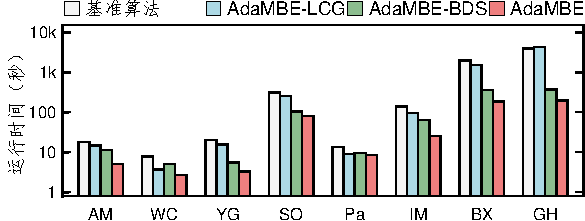
\includegraphics[width=0.8\linewidth]{adambe/breakdown_time}
		\label{fig:ada_breakdown_time}
	}
	\\
  \subfloat[内存使用评估]{
		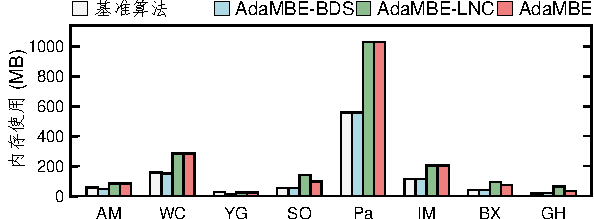
\includegraphics[width=0.8\linewidth]{adambe/breakdown_memory}
		\label{fig:ada_breakdown_memory}
	}

  \caption{BDS、LNC方法的运行时间与内存使用细分评估}
  \label{fig:ada_breakdown}
\end{figure}

\textbf{运行时间和内存使用评估:} 我们在包含更多极大二分图计数的8个常规数据集上评估了运行时间和内存使用情况。根据图~\ref{fig:ada_breakdown_time} 的展示结果,BDS 和 LNC 优化总是能够加速基准算法,而 AdaMBE 结合这两种优化而获得优于其他变体的性能。值得注意的是,在 Github 数据集上,AdaMBE 将基准算法的运行时间从 3,911 秒缩短至 194 秒。此外,从图~\ref{fig:ada_breakdown_memory} 可以看出,由于在运行时动态存储局部邻居,LNC 增加了内存使用量。但是由于极大二分团枚举是一个计算密集型问题,内存需求相对较低,因此增加一定的内存使用来加速计算过程是一个合算的策略。综合而言,在所有测试数据集上,AdaMBE 的内存使用不超过1.3 GB(在 CebWiki 数据集上),总体来说是可以接受的。

\begin{figure} [H]
	\centering
  % \vspace{0.05in}
	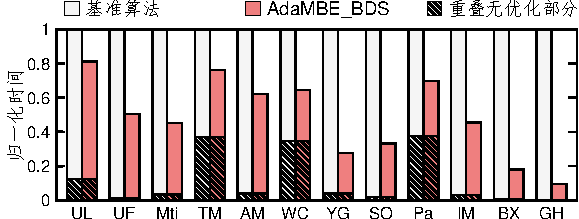
\includegraphics[width=0.8\linewidth]{adambe/breakdown_design1}
  % \vspace{0.05in}
	\caption{BDS方法下的运行时间分解分析}

	\label{fig:ada_breakdown_design1}
\end{figure}

\textbf{BDS方法的效果:} 为了研究在第~\ref{subsec:ada_design_1}节提出的 BDS 方法的效果,我们对基准算法和AdaMBE-BDS进行了运行时间分解分析,如图~\ref{fig:ada_breakdown_design1}所示。考虑到 BDS 方法仅对$|L|$等于或小于阈值$\tau$的小节点$(L, R, C)$进行优化,为了便于清晰比较,图中标记了基准算法与AdaMBE-BDS重叠的无优化部分,即大节点初始化和计算的重叠时间。结果显示,BDS 方法在大多数数据集中将小节点的计算时间缩短了50\%以上。值得注意的是,在Github数据集上,BDS 实现了显著的91\%减少,导致AdaMBE-BDS相对于基准算法加速了10.7倍。

\begin{figure} [H]
	\centering
  % \vspace{0.05in}
	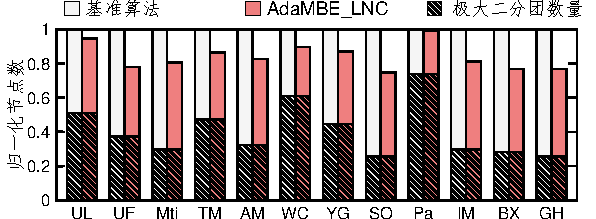
\includegraphics[width=0.8\linewidth]{adambe/breakdown_design2}
  % \vspace{0.05in}
	\caption{LNC方法的节点剪枝效率}

	\label{fig:ada_breakdown_design2}
\end{figure}

\textbf{LNC方法的效果:} 为了评估LNC方法的影响,我们探讨了在第~\ref{subsec:ada_design_2}节提到的三种冗余的减少效果。关于节点级别的粗粒度冗余,图~\ref{fig:ada_breakdown_design2}显示LNC方法平均减少了25\%的包含非极大二分团的节点。在集合操作级别的中等粒度冗余方面,LNC利用局部邻居缓存避免了重新计算集合$L$,从而完全消除了这种冗余。至于顶点级别的细粒度冗余,~\ref{subsec:ada_limitation}节的表~\ref{tbl:ada_motivation}显示,LNC方法在大多数数据集中减少了超过90\%的无关顶点访问。与之前只处理粗粒度冗余(即非极大二分团)的方法不同,LNC方法通过处理所有三种类型的冗余,提高了性能。

\subsection{敏感性测试}
\label{subsec:ada_eval_sensitivity}

我们对BDS方法中的阈值$\tau$选择、顶点的顺序选择以及算法的可扩展性进行了敏感性测试。


\begin{figure} [H]
	\centering
  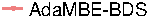
\includegraphics[width=0.2\linewidth]{adambe/sensitivity_threshold_legend} \\
  \subfloat[BookCrossing.]{
		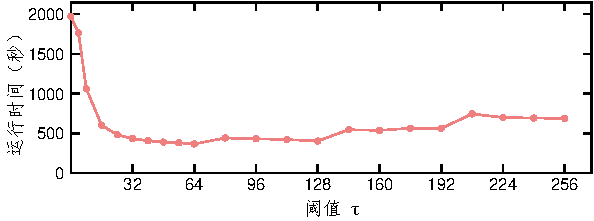
\includegraphics[width=0.8\linewidth]{adambe/sensitivity_threshold_bx}
		\label{fig:sensitivity_threshold_bx}
	}
	\\
  \subfloat[Github.]{
		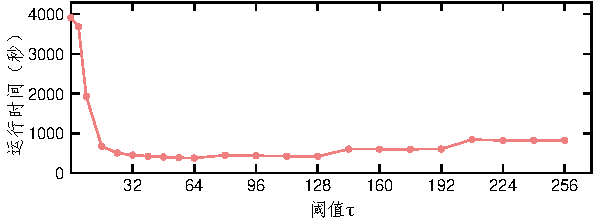
\includegraphics[width=0.8\linewidth]{adambe/sensitivity_threshold_gh}
		\label{fig:sensitivity_threshold_gh}
	}

	\caption{不同阈值$\tau$下BDS方法性能评估}
	\label{fig:ada_sensitivity_threshold}

\end{figure}

\textbf{BDS方法中阈值$\tau$的影响:}为确定第~\ref{subsec:ada_design_1}节中的阈值$\tau$,我们在AdaMBE-BDS上进行了不同$\tau$值(从4到256)的实验,该实验仅启用了BDS方法。图~\ref{fig:ada_sensitivity_threshold}展示了来自两个较大的常规数据集(即BookCrossing和Github)的实验结果。当$\tau$从4增加到64时,运行时间持续减少,因为较大的$\tau$导致创建的子图减少,并且位图的重用增加。值得注意的是,由于当$\tau$不大于64时,每次集合交集只需要对两个64位长整数进行一次按位AND操作,因此集合交集时间保持不变。然而,当$\tau$超过64时,由于每次集合交集所需的时间增加,运行时间变得更长。此外,我们注意到当$\tau$是64的倍数时,运行时间较短,因为这些情况增强了位图的重用,并且每次集合交集所需时间相同。因此,AdaMBE将$\tau$的默认值设定为64。


\begin{figure} [H]
	\centering
  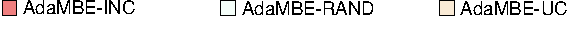
\includegraphics[width=0.8\linewidth]{adambe/order_legend}
  

  % \subfigure[Medium datasets.]{
		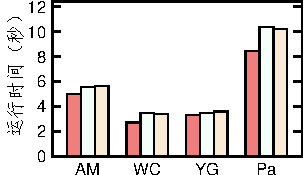
\includegraphics[width=0.42\linewidth]{adambe/order_medium}
	% }
  \quad
  % \subfigure[Large datasets.]{
		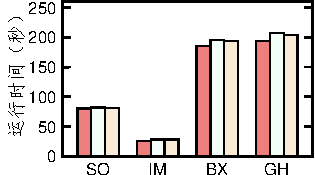
\includegraphics[width=0.42\linewidth]{adambe/order_large}
	% }

	\caption{顶点顺序的性能评估}
	\label{fig:ada_order}

\end{figure}

\textbf{顶点排序的影响:} 为确定AdaMBE算法的顶点初始排序,我们设计了三种变体:AdaMBE-INC、AdaMBE-RAND和AdaMBE-UC。其中,AdaMBE-INC 根据邻居数量递增对顶点进行排序。 AdaMBE-RAND以随机顺序对顶点进行排序。 AdaMBE-UC使用了最近工作ooMBEA~\cite{ooMBE22}提出的单方面顺序。 图~\ref{fig:ada_order}显示,在8个较大的常规数据集上,AdaMBE-INC始终优于AdaMBE-RAND和AdaMBE-UC。因此,AdaMBE的默认顶点排序是基于邻居数量递增的。


\begin{figure} [H]
	\centering
		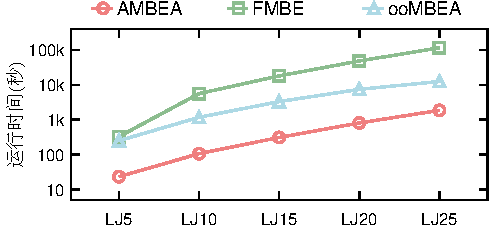
\includegraphics[width=0.8\linewidth]{adambe/scalability}
	\caption{可扩展性评估(对数形式)}
	\label{fig:ada_scalability}
\end{figure}


\textbf{可扩展性评估:} 我们使用从包含超过1亿条边的LiveJournal数据集生成的合成数据集来评估AdaMBE的可扩展性。本实验中,我们从LiveJournal中抽样10\%、20\%、30\%、40\%和50\%的边,并将它们分别命名为LJ10、LJ20、LJ30、LJ40和LJ50。表~\ref{tbl:ada_datasets}总结了这些数据集的统计信息。图~\ref{fig:ada_scalability}显示,在所有合成数据集上,AdaMBE比所有串行竞争对手快11.4倍以上。具体而言,仅需6.6小时,AdaMBE就可以在包含超过60亿个极大二分团的LJ50上完成MBE计算,而其他竞争对手无法在48小时内完成。实验结果表明,AdaMBE是处理大型数据集的最佳选择。

\section{本章小结}

本章提出了基于位图的动态子图(BDS)方法和局部邻居缓存(LNC)方法,并结合这两种方法形成高效的极大二分团枚举算法AdaMBE。旨在解决极大二分团枚举问题中计算不规则、单一数据结构低效的挑战。首先,针对邻接表上集合运算的高开销问题,BDS方法在计算过程中动态生成子位图,以加速集合运算。通过利用位运算在子位图中进行集合运算,提升了效率。其次,针对现有方法中访问顶点完整邻居导致的冗余计算问题,LNC方法仅动态保存顶点的部分对计算结果有影响的活跃邻居,避免了大量对结果无影响的不活跃邻居的访问,从而减少了枚举节点层面、集合运算层面和顶点访问层面三种粒度的冗余计算。最后,将这两种技术整合,实现了AdaMBE算法及其并行版本ParAdaMBE。实验结果充分证明了AdaMBE算法的高性能,以及本章中所有优化方法的具体作用。